\documentclass[12pt]{article}

\usepackage{extsizes}
\usepackage{graphicx}
\usepackage{listings}
\usepackage{color}
\usepackage{hyperref}
\usepackage{float}
\usepackage{amsmath}
\usepackage{amssymb}
\usepackage{cite}
\usepackage[justification=centering]{caption}
\usepackage{microtype}
\usepackage{xcolor}

\definecolor{codegreen}{rgb}{0,0.6,0}
\definecolor{codegray}{rgb}{0.5,0.5,0.5}
\definecolor{codepurple}{rgb}{0.58,0,0.82}
\definecolor{backcolour}{rgb}{0.95,0.95,0.92}

\lstdefinestyle{mystyle}{
    backgroundcolor=\color{backcolour},   
    commentstyle=\color{codegreen},
    keywordstyle=\color{magenta},
    numberstyle=\tiny\color{codegray},
    stringstyle=\color{codepurple},
    basicstyle=\ttfamily\footnotesize,
    breakatwhitespace=false,         
    breaklines=true,                 
    captionpos=b,                    
    keepspaces=true,                 
    numbers=left,                    
    numbersep=5pt,                  
    showspaces=false,                
    showstringspaces=false,
    showtabs=false,                  
    tabsize=2
}
\lstset{style=mystyle}

\usepackage[a4paper,bottom=30mm,left=25mm,right=25mm,top=30mm]{geometry}

\hypersetup{colorlinks=false,pdfborder={0 0 0}}

\begin{document}

\title{CS406 Course Project \\ \textbf{Shor's and other interesting Quantum Algorithms}}
\author{Dhananjay Raman\hspace{3.5cm}Tanay Vineet Tayal \\ 210050044\hspace{5.7cm}210050155}
\date{3 May 2024}

\maketitle
\tableofcontents
\section{Problem Description}
Many encryption systems, like the RSA scheme, which is one of the cornerstones of modern cryptography, rely on the difficulty of prime factorization of large numbers into their prime components\cite{rsa}. The security of these systems is based on the assumption that no efficient classical algorithm exists for factorization. The best classical algorithms for factoring large numbers grow sub-exponentially with the size of the numbers, making it computationally impractical for very large numbers \cite{classical}. This computational challenge is crucial in maintaining the security of modern cryptography.
\par\noindent Quantum computers are different from classical computers, utilizing quantum mechanical principles like superposition and entanglement. Quantum computers have the potential to solve certain problems much more efficiently (even exponential speedup is possible). \textbf{Shor's Algorithm} \cite{shor} poses a theoretical threat to the foundation of current cryptographic practices by promising an efficient method for factoring large numbers.

\section{Shor's Algorithm}
\subsection{Overview}
Shor's Algorithm is a quantum algorithm for integer factorization. It is a polynomial-time quantum algorithm that can factorize an integer $N$ into its prime factors in $O((\log N)^3)$ time. The algorithm consists of two main parts:
\begin{enumerate}
    \item \textbf{Classical Reduction}: Reduce the problem of factoring $N$ to the problem of finding the period of a function.
    \item \textbf{Quantum Subroutine}: Use a quantum subroutine to find the period of a function.
\end{enumerate}
\par\noindent At the heart of Shor's Algorithm we have the problem of finding the period of a function. The specific function used in Shor's Algorithm is the \textbf{Modular Exponentiation Function}:
$$f(x) = a^x \mod N$$
where $a$ is a randomly chosen integer between $1$ and $N-1$ and $N$ is the number to be factorized. The \textit{order} or \textit{period} of the function $f(x)$ is the smallest positive integer $r$ such that $a^r \mod N = 1$. The period of the function $f(x)$ is crucial in the factorization of $N$. It has the following properties:
\begin{enumerate}
    \item $f(x+r) = f(x) \quad \forall x \in \mathbb{Z}$
    \item If $r$ is even, then $a^r-1$ can be factored as $(a^{r/2}-1)(a^{r/2}+1)$, and since $N$ divides $a^r-1$, $N$ shares common factors with $(a^{r/2}-1)$ and $(a^{r/2}+1)$.
\end{enumerate}
\par\noindent The algorithm is probabilistic and requires a quantum computer to perform the quantum subroutine. The algorithm has been proven to run in polynomial time on a quantum computer, but the practical implementation of the algorithm is still a challenge due to the error rates in quantum computers.
\par\noindent \textbf{Note:} For demonstration (and implementation) purposes, we describe the quantum circuit for a small number $N=15$.

\subsection{Classical Reduction}
The classical reduction part of Shor's Algorithm involves reducing the problem of factoring $N$ to the problem of finding the period of a function. The steps involved in the classical reduction are as follows:
\begin{enumerate}
    \item Choose a random integer $a$ between $1$ and $N-1$.
    \item Compute the greatest common divisor of $a$ and $N$. If $1 < \text{gcd}(a, N) < N$, then the greatest common divisor is a non-trivial factor of $N$.
    \item If the greatest common divisor is a non-trivial factor of $N$, then the factorization is complete, and the algorithm returns the factors.
    \item If the greatest common divisor is $1$, then proceed to the quantum subroutine to find the period of the function $f(x) = a^x \mod N$.
    \item If the period of the function is even, then compute $g=\text{gcd}(a^{r/2}+1, N)$. If $g$ is non-trivial, then the algorithm returns the factors $g$ and $N/g$.
    \item If the period of the function is odd or $g$ is trivial, then repeat the process with a different random integer $a$.
\end{enumerate}
The pseudocode for the classical reduction part of Shor's Algorithm is as follows:
\begin{lstlisting}[language=Python, caption=Core Algorithm]
def shor(N):
    while True:
        a = random.randint(1, N-1)
        g = gcd(a, N)
        if 1 < g < N:
            return g, N//g
        if g == N:
            continue
        r = find_period(a, N)
        if r % 2 == 0:
            g = gcd(a**(r//2)+1, N)
            if 1 < g < N:
                return g, N//g
\end{lstlisting}

\subsection{Quantum Subroutine}
The quantum subroutine part of Shor's Algorithm involves finding the period of the function $f(x) = a^x \mod N$. The quantum subroutine uses the Quantum Fourier Transform (QFT) to find the period of the function.
\begin{figure}[H]
    \centering
    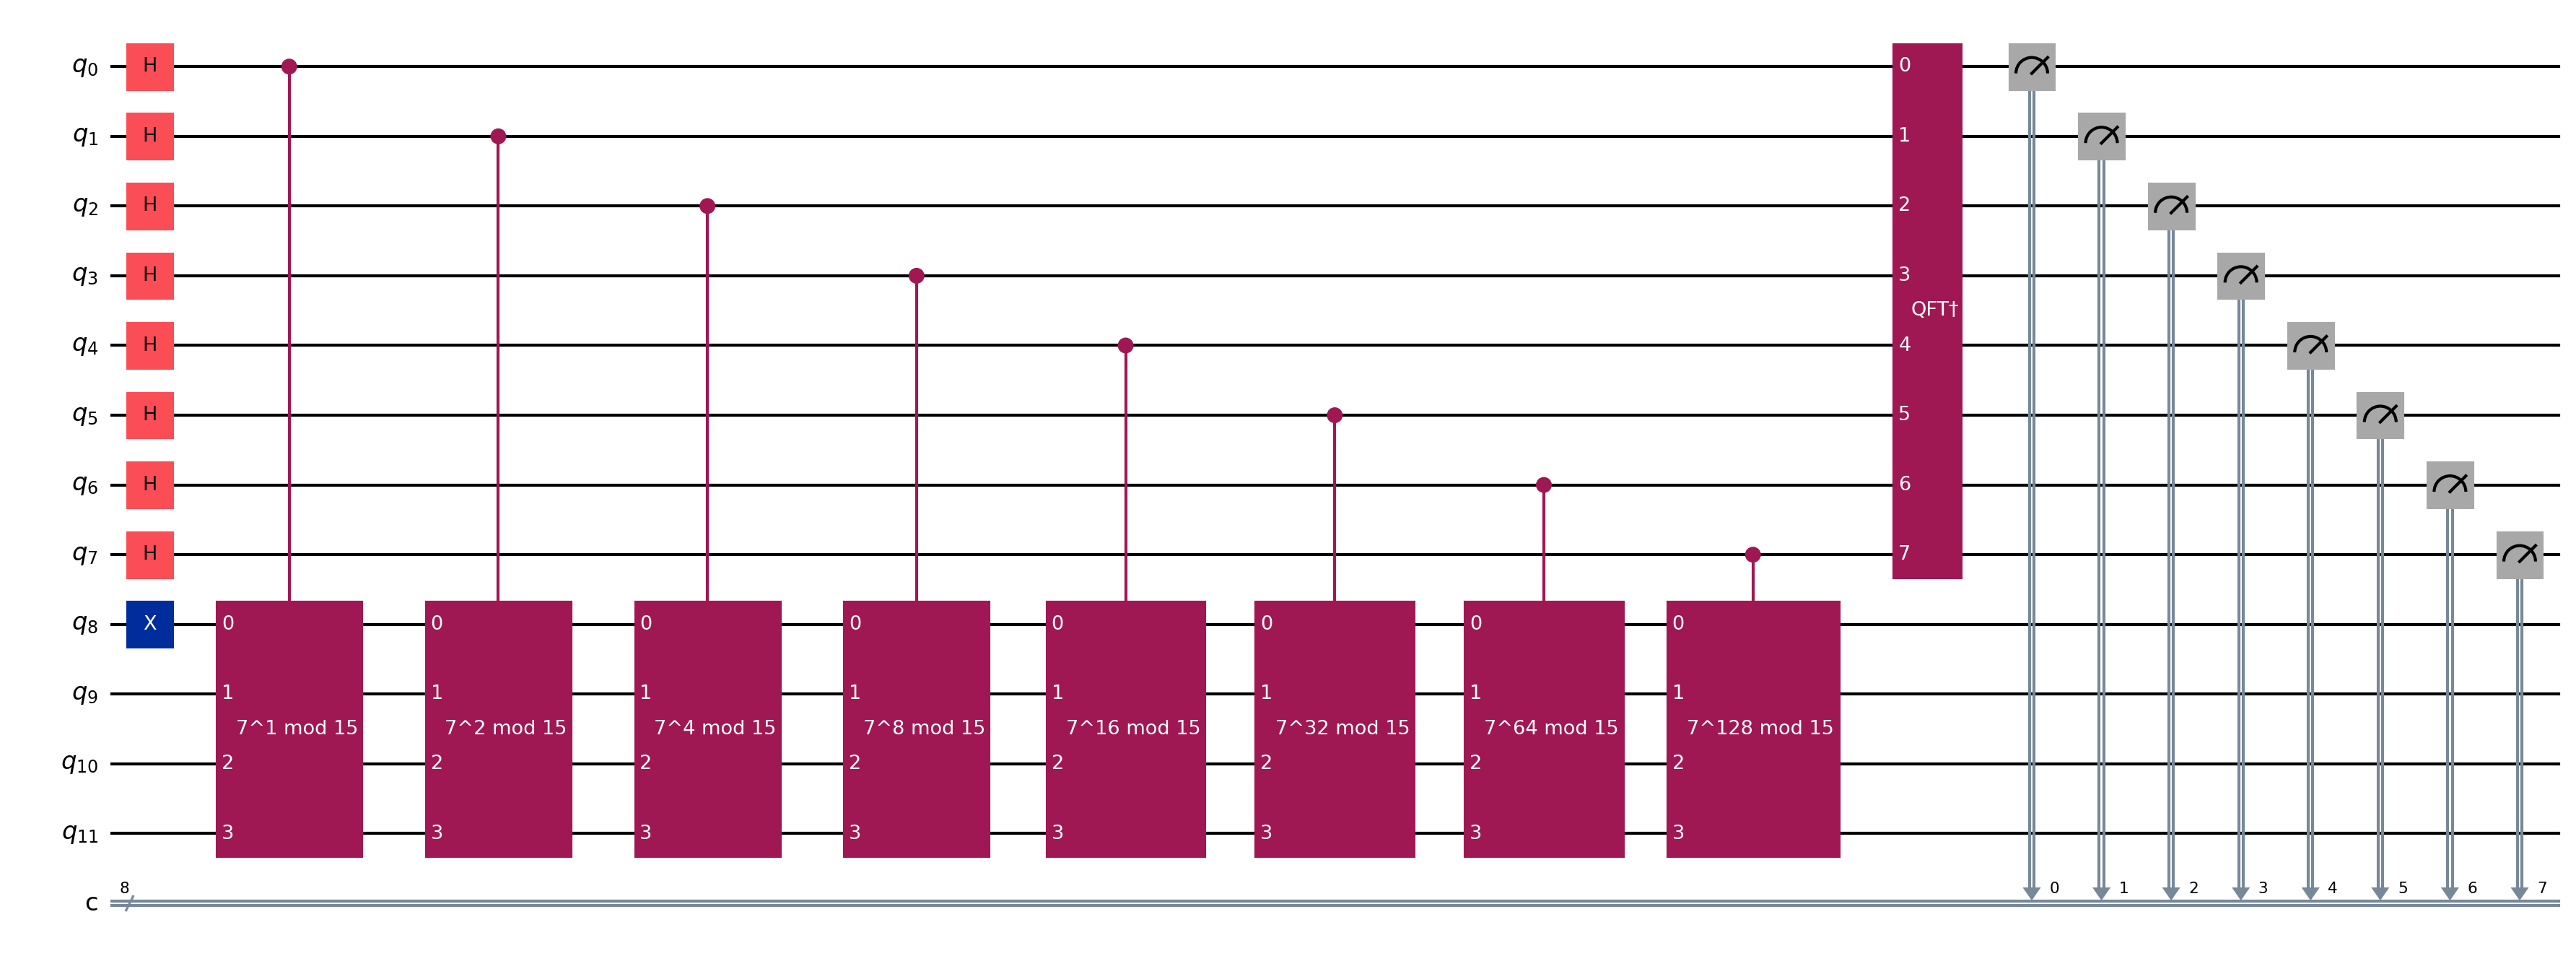
\includegraphics[height=0.53\textwidth, angle=-90,origin=c]{../shors.png}
    \caption{Quantum Circuit for Shor's Algorithm (for $N=15$) in Qiskit \cite{qiskit}.}
\end{figure}
\par\noindent The main steps involved in the quantum subroutine are as follows:
\begin{enumerate}
    \item \textbf{Register Initialization}: We initialize three registers:
    \begin{enumerate}
        \item A register of size $l$ qubits (\texttt{q0} - \texttt{q7}) which will serve as the input to the Quantum Fourier Transform. These qubits are prepared in the superposition of all possible states using Hadamard (H) gates. Here $l$ should be chosen such that $2^l > N^2$, so that the period can be used to accurately determine the factors of $N$.
        \item A register of size $n$ qubits (\texttt{q8} - \texttt{q11}) which will be used to perform the modular exponentiation. Here, $n=\log_2 N$ is the number of bits required to represent $N$.
        \item A third classical register (\texttt{c}) to store the results of the measurements.
    \end{enumerate}
    \item \textbf{Modular Exponentiation}: The sequence of blocks labeled with $f(x) = 7^{2^i} \mod 15$ (where $i$ ranges from $0$ to $7$) represent the modular exponentiation operation. The modular exponentiation is performed by applying controlled-$U$ gates, where $U$ is the unitary operator for the function $f(x) = a^x \mod N$. The unitary operator $U$ is defined as:
    $$U|y\rangle|0\rangle = |y\rangle|a^y \mod N\rangle$$
    This operation is controlled by the qubits in the first register and the result is stored in the second register, and creates a highly entangled state where the second register contains the values of $a^x \mod N$ for all $x$, $x$ being the state represented by the qubits \texttt{q0} - \texttt{q7} in the first register.
    \item \textbf{Quantum Fourier Transform}: The Quantum Fourier Transform is applied to the first register to find the period of the function. The Quantum Fourier Transform is a quantum analogue of the Discrete Fourier Transform and is used to find the period of a function in superposition. The Quantum Fourier Transform is implemented using a series of Hadamard gates and controlled-phase gates.
    \item \textbf{Measurement}: The first register is measured, i.e. the qubits \texttt{q0} - \texttt{q7} are measured, and the result is stored in the classical register \texttt{c}.
    \item \textbf{Period Extraction}: The final measurement (of register \texttt{c}) gives an 8-bit string. This 8-bit string is converted from binary and divided by $2^8=256$ to get the phase as a fraction $s/r$, where $s$ is a random integer between $0$ and $r-1$ and $r$ is the period/order of the function. Thus after rationalizing the fraction, the denominator $r$ gives a "guess" for the period $r$ of the function, and is returned to the classical reduction part of the algorithm.
\end{enumerate}

\subsection{Code Implementation}
The code for the quantum subroutine of Shor's Algorithm for $N=15$ is implemented using Qiskit, an open-source quantum computing framework \cite{qiskit}. All the code for the quantum subroutine is available in the Jupyter Notebook \texttt{shors.ipynb} in the repository. The code can be run on a quantum simulator or a real quantum computer using IBM Quantum Experience. Link for the repository: \url{https://github.com/Seraphsnow/CryptoProject-}

\subsection{Caveats}
\begin{enumerate}
    \item \textbf{Probabilistic}: The algorithm may require multiple runs to find the correct factors.
    \item \textbf{Requirement of a large Quantum Computer}: The algorithm requires a large number of qubits to factor numbers of a practical size (such as 2048-bit numbers used in RSA). The current state of quantum computers is not sufficient to factor such large numbers.
    \item \textbf{Error Rates and Quantum Decoherence}: Quantum Computers are prone to errors due to noise and decoherence (loss of quantum information from interaction of system with environment), which can affect the fidelity (amount of information preserved) of the quantum computation. The quantum gates must operate with very high precision, and maintaining coherence for the required number of qubits over the time is a significant challenge.
\end{enumerate}

\subsection{Variants}
\begin{enumerate}
    \item \textbf{Shor's Algorithm for the Discrete Log Problem}: Shor's Algorithm can also be used to solve the discrete logarithm problem \cite{dl}, which is the basis of many cryptographic schemes like the Diffie-Hellman key exchange and the Digital Signature Algorithm. The algorithm works by finding the period of a function similar to the modular exponentiation function used in integer factorization:
    $$f(x) = g^x \mod p$$
    where $g$ is a generator of the group and $p$ is a prime number. The period of the function is used to find the discrete logarithm of $g$ with respect to $p$. Again, we reduce the problem to finding the period of the function and use the Quantum Fourier Transform/Phase Estimation to find the period.
    \item \textbf{Generalization to the Hidden Subgroup Problem}: Shor's Algorithm can be generalized to solve the Hidden Subgroup Problem, which is a generalization of problems like the discrete logarithm problem and the integer factorization problem. The Hidden Subgroup Problem is a computational problem that arises in the study of quantum algorithms and has applications in cryptography and number theory.
    \par\noindent Given a group $G$ and a function $f: G \rightarrow X$, the goal is to find the hidden subgroup $H$ of $G$ such that $f$ is constant on the cosets of $H$. For any finite \textit{abelian} group $G$, the Hidden Subgroup Problem can be solved efficiently using quantum algorithms based on Shor's Algorithm \cite{qcqi}.
\end{enumerate}

\section{Other Quantum Algorithms}
This section describes some other interesting quantum algorithms relevant to cryptography, mentioned here to generate interest in the reader. 
\subsection{Grover's Algorithm}
Grover's Algorithm is a quantum algorithm for searching an unsorted database\cite{grover}. The algorithm provides a \textbf{quadratic speedup} over the best classical algorithms for the same problem. The algorithm has applications in searching, optimization, and cryptography. The algorithm works by iteratively applying a sequence of quantum operations to amplify the probability of finding the correct solution. The algorithm has been proven to run in $O(\sqrt{N})$ time on a quantum computer, where $N$ is the size of the database.
\par\noindent Grover's Algorithm can be used to solve the problem of finding the pre-image of a hash function in $O(\sqrt{N})$ time, where $N$ is the size of the hash function's output. This has implications for cryptographic hash functions and digital signatures, as it effectively reduces the security of $n$-bit hash functions to $n/2$ bits in the quantum setting.

\subsection{Quantum Key Distribution (BB84 Protocol)}
Quantum Key Distribution (QKD) is a secure communication method that uses quantum mechanics to secure a communication channel. The BB84 Protocol is a quantum key distribution protocol that allows two parties to securely establish a shared secret key\cite{bb84}. The security of the protocol is based on the principles of quantum mechanics, such as the no-cloning theorem and the uncertainty principle. The protocol uses the properties of quantum states to detect eavesdropping and ensure the security of the communication channel.
\par\noindent The BB84 Protocol is used in quantum cryptography to secure communication channels and is the basis for many quantum key distribution systems. The protocol has been implemented in various quantum communication systems and has been shown to be secure against various types of attacks.

\begin{thebibliography}{00}
    \bibitem{rsa} R. L. Rivest, A. Shamir, and L. Adleman. 1978. A method for obtaining digital signatures and public-key cryptosystems. Commun. ACM 21, 2 (Feb. 1978), 120-126. https://doi.org/10.1145/359340.359342
    \bibitem{classical} Buhler, J.P., Lenstra, H.W., Pomerance, C. (1993). Factoring integers with the number field sieve. In: Lenstra, A.K., Lenstra, H.W. (eds) The development of the number field sieve. Lecture Notes in Mathematics, vol 1554. Springer, Berlin, Heidelberg. https://doi.org/10.1007/BFb0091539
    \bibitem{shor} P. W. Shor, "Algorithms for quantum computation: discrete logarithms and factoring," Proceedings 35th Annual Symposium on Foundations of Computer Science, Santa Fe, NM, USA, 1994, pp. 124-134, doi: 10.1109/SFCS.1994.365700.
    \bibitem{qiskit} Gadi Aleksandrowicz, Thomas Alexander, Panagiotis Barkoutsos, Luciano Bello, Yael Ben-Haim, David Bucher, Francisco Jose Cabrera-Hernández, Jorge Carballo-Franquis, Adrian Chen, Chun-Fu Chen, Jerry M. Chow, Antonio D. Córcoles-Gonzales, Abigail J. Cross, Andrew Cross, Juan Cruz-Benito, Chris Culver, Salvador De La Puente González, Enrique De La Torre, Delton Ding, … Christa Zoufal. (2019). Qiskit: An Open-source Framework for Quantum Computing (0.7.2). Zenodo. https://doi.org/10.5281/zenodo.2562111
    \bibitem{dl} Peter W. Shor. 1997. Polynomial-Time Algorithms for Prime Factorization and Discrete Logarithms on a Quantum Computer. SIAM J. Comput. 26, 5 (Oct. 1997), 1484–1509. https://doi.org/10.1137/S0097539795293172
    \bibitem{qcqi} Michael A. Nielsen and Isaac L. Chuang. 2010. Quantum Computation and Quantum Information: 10th Anniversary Edition (10th ed.). Cambridge University Press, New York, NY, USA.
    \bibitem{grover} L.~K.~Grover,
    ``A Fast quantum mechanical algorithm for database search,''
    [arXiv:quant-ph/9605043 [quant-ph]].
    \bibitem{bb84} Bennett, Charles \& Brassard, Gilles. (1984). WITHDRAWN: Quantum cryptography: Public key distribution and coin tossing. Theoretical Computer Science - TCS. 560. 175-179. 10.1016/j.tcs.2011.08.039.
\end{thebibliography}
\end{document}